\documentclass[border=8pt]{standalone}
\usepackage{fontspec}
\defaultfontfeatures{Ligatures=TeX}
\setmainfont{Palatino Linotype}
\setsansfont{Arial}
\usepackage{amsmath,amssymb}
\usepackage{tikz}
\usetikzlibrary{arrows.meta,positioning,calc,shapes.geometric,fit}
\definecolor{tksInk}{HTML}{1C1A16}
\definecolor{tksMuted}{HTML}{8A8378}
\definecolor{tksAccent}{HTML}{8C5A1F}
\definecolor{tksAfill}{HTML}{F6EEDD}
\definecolor{tksAedge}{HTML}{9A7328}
\definecolor{tksBfill}{HTML}{E6EDF5}
\definecolor{tksBedge}{HTML}{2F5B85}
\definecolor{tksCfill}{HTML}{F7E7E4}
\definecolor{tksCedge}{HTML}{95403A}
\definecolor{tksDfill}{HTML}{E4EFE6}
\definecolor{tksDedge}{HTML}{3A6B45}
\definecolor{tksEfill}{HTML}{F5DFDC}
\definecolor{tksEedge}{HTML}{A33B30}
\begin{document}
\centering
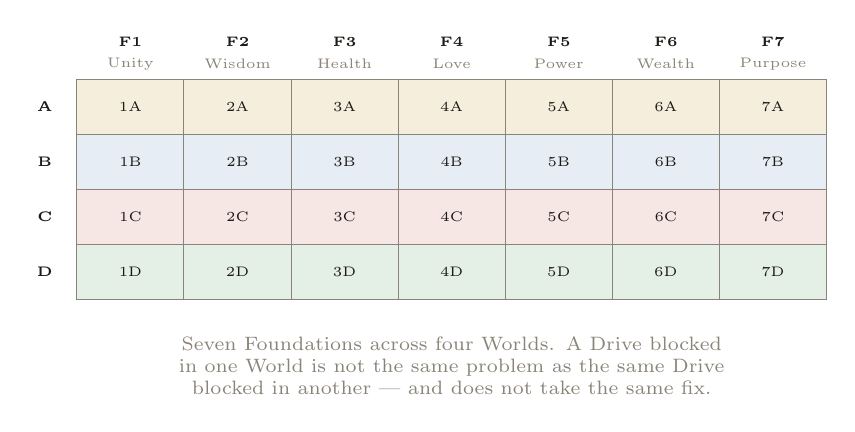
\begin{tikzpicture}[x=13.6mm, y=7.0mm, font=\sffamily]
  \foreach \c/\f/\nm in {0/F1/Unity, 1/F2/Wisdom, 2/F3/Health, 3/F4/Love,
                         4/F5/Power, 5/F6/Wealth, 6/F7/Purpose} {
    \node[font=\tiny\bfseries, text=tksInk] at (\c+0.5, 0.68) {\f};
    \node[font=\tiny, text=tksMuted] at (\c+0.5, 0.28) {\nm};
  }
  \foreach \r/\w/\f in {0/A/tksAfill, 1/B/tksBfill, 2/C/tksCfill, 3/D/tksDfill} {
    \node[font=\tiny\bfseries, text=tksInk] at (-0.3, -\r-0.5) {\w};
    \foreach \c in {0,...,6} {
      \draw[draw=tksMuted, line width=0.35pt, fill=\f]
        (\c, -\r) rectangle (\c+1, -\r-1);
      \pgfmathtruncatemacro\num{\c+1}
      \node[font=\tiny, text=tksInk] at (\c+0.5, -\r-0.5) {\num\w};
    }
  }
  \node[anchor=north, text width=88mm, align=center, font=\scriptsize,
        text=tksMuted] at (3.5, -4.5)
    {Seven Foundations across four Worlds. A Drive blocked in one World is not
     the same problem as the same Drive blocked in another --- and does not
     take the same fix.};
\end{tikzpicture}
\end{document}
